\section{後処理と描画} \label{sec:ideal_exp_net2g}
%------------------------------------------------------
ここでは後処理と計算結果の描画方法を説明する。このチュートリアルでは、
{\netcdf}形式の分散ファイルを単一のファイルに結合し、ダイレクトアクセスが可能な
単純なバイナリ形式(\grads 形式)に変換する。
このバイナリ形式は、ユーザーによる結果の解析を容易にする。
まず、\ref{sec:source_net2g}節でコンパイルした後処理ツール\verb|net2g|へのリンクを張る。
\begin{verbatim}
  $ ln -s ../../../util/netcdf2grads_h/net2g  ./
\end{verbatim}

\verb|net2g| の実行方法は、基本的に{\scalerm}と同じであり、
\begin{verbatim}
  $ mpirun  -n  [プロセス数]  ./net2g  [設定ファイル]
\end{verbatim}
の形式で実行する。
\verb|net2g_R20kmDX500m.conf|は\verb|net2g| 専用の設定ファイルである。
この設定ファイルを\verb|net2g|に与えて、次のように実行する。
\begin{verbatim}
  $ mpirun  -n  2  ./net2g  net2g_R20kmDX500m.conf
\end{verbatim}
エラーメッセージがなく、下記のメッセージだけが標準出力へ表示されていれば、変換は正常に完了している。
\msgbox{
\verb|+++ MPI COMM: Corrective Finalize| \\
}

\verb|net2g|を実行する際には、{\scalerm}の実行時に使用した MPI プロセス数と同じか、
その約数のプロセス数を使用しなければならない。
%HDDの読み書き速度に依存するが、本書の必要要件にあった計算機であれば2分程度で計算が終わる。
この実行によって、実行ディレクトリ下に下記の 6 つのファイルが作成される。
\begin{alltt}
  QHYD_d01z-3d.ctl
  QHYD_d01z-3d.grd
  U_d01z-3d.ctl
  U_d01z-3d.grd
  W_d01z-3d.ctl
  W_d01z-3d.grd
\end{alltt}
「grd」ファイルは、分割ファイルを結合することによって得られる、
ダイレクトアクセス可能な単純バイナリ形式(\grads 形式)である。
一方で、「ctl」ファイルは \grads によって「grd」ファイルを読む込むときに必要な情報を含む。

計算が問題なく完了しているかを確認するため、\grads スクリプト \verb|checkfig_ideal.gs|
を使って作図する。なお、\grads のバージョンによって文法が異なるため、
警告が出る場合には\grads スクリプトを適宜変更されたい。
作図は以下のコマンドで行う。
\begin{verbatim}
  $ grads -blc checkfig_ideal.gs
\end{verbatim}
コマンドが成功すれば、下記のファイルが生成される。
\begin{verbatim}
   ideal_QHYD.png
   ideal_W.png
\end{verbatim}
シミュレーションと後処理が問題なく行われていれば、図\ref{fig_ideal}と同じ図が得られる。

\begin{figure}[t]
\begin{center}
  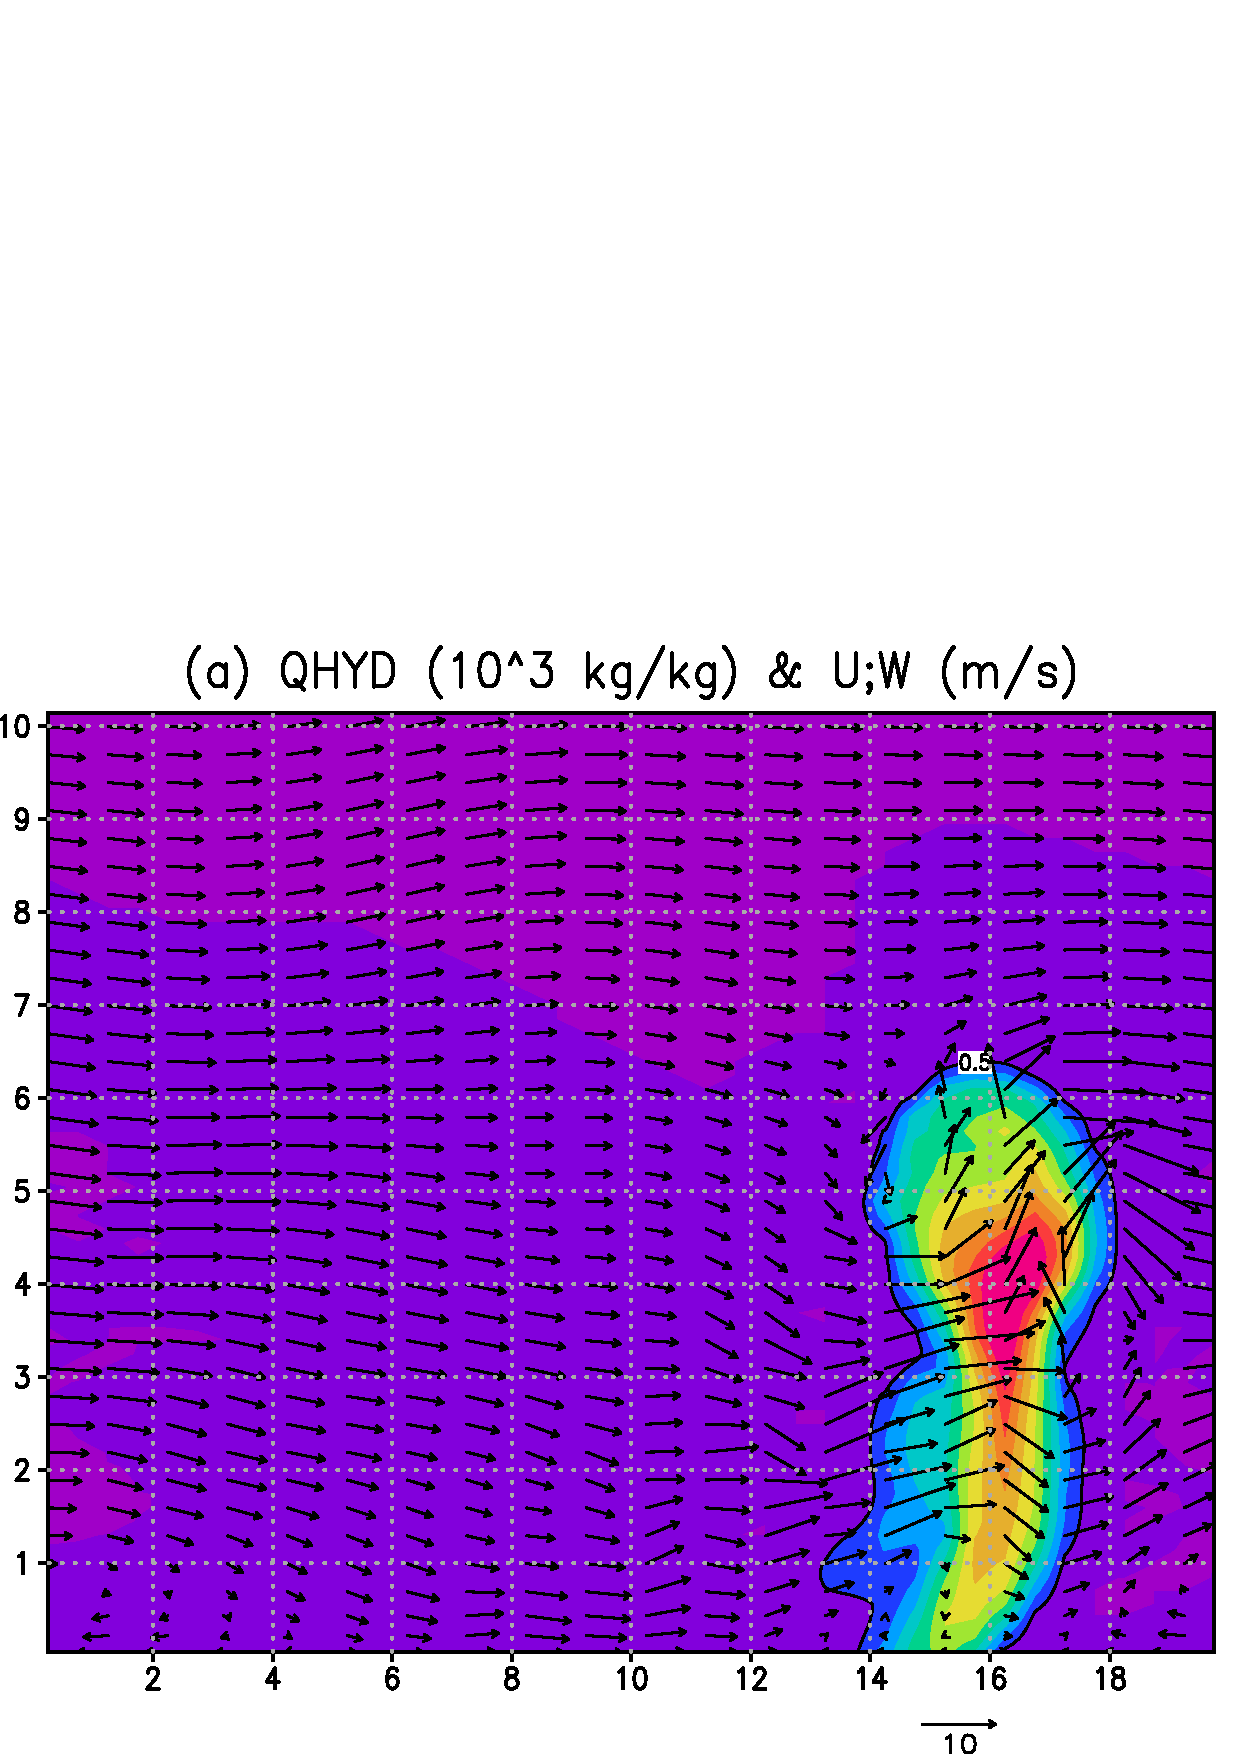
\includegraphics[width=0.7\hsize]{./figure/ideal_qhyd.pdf}\\
  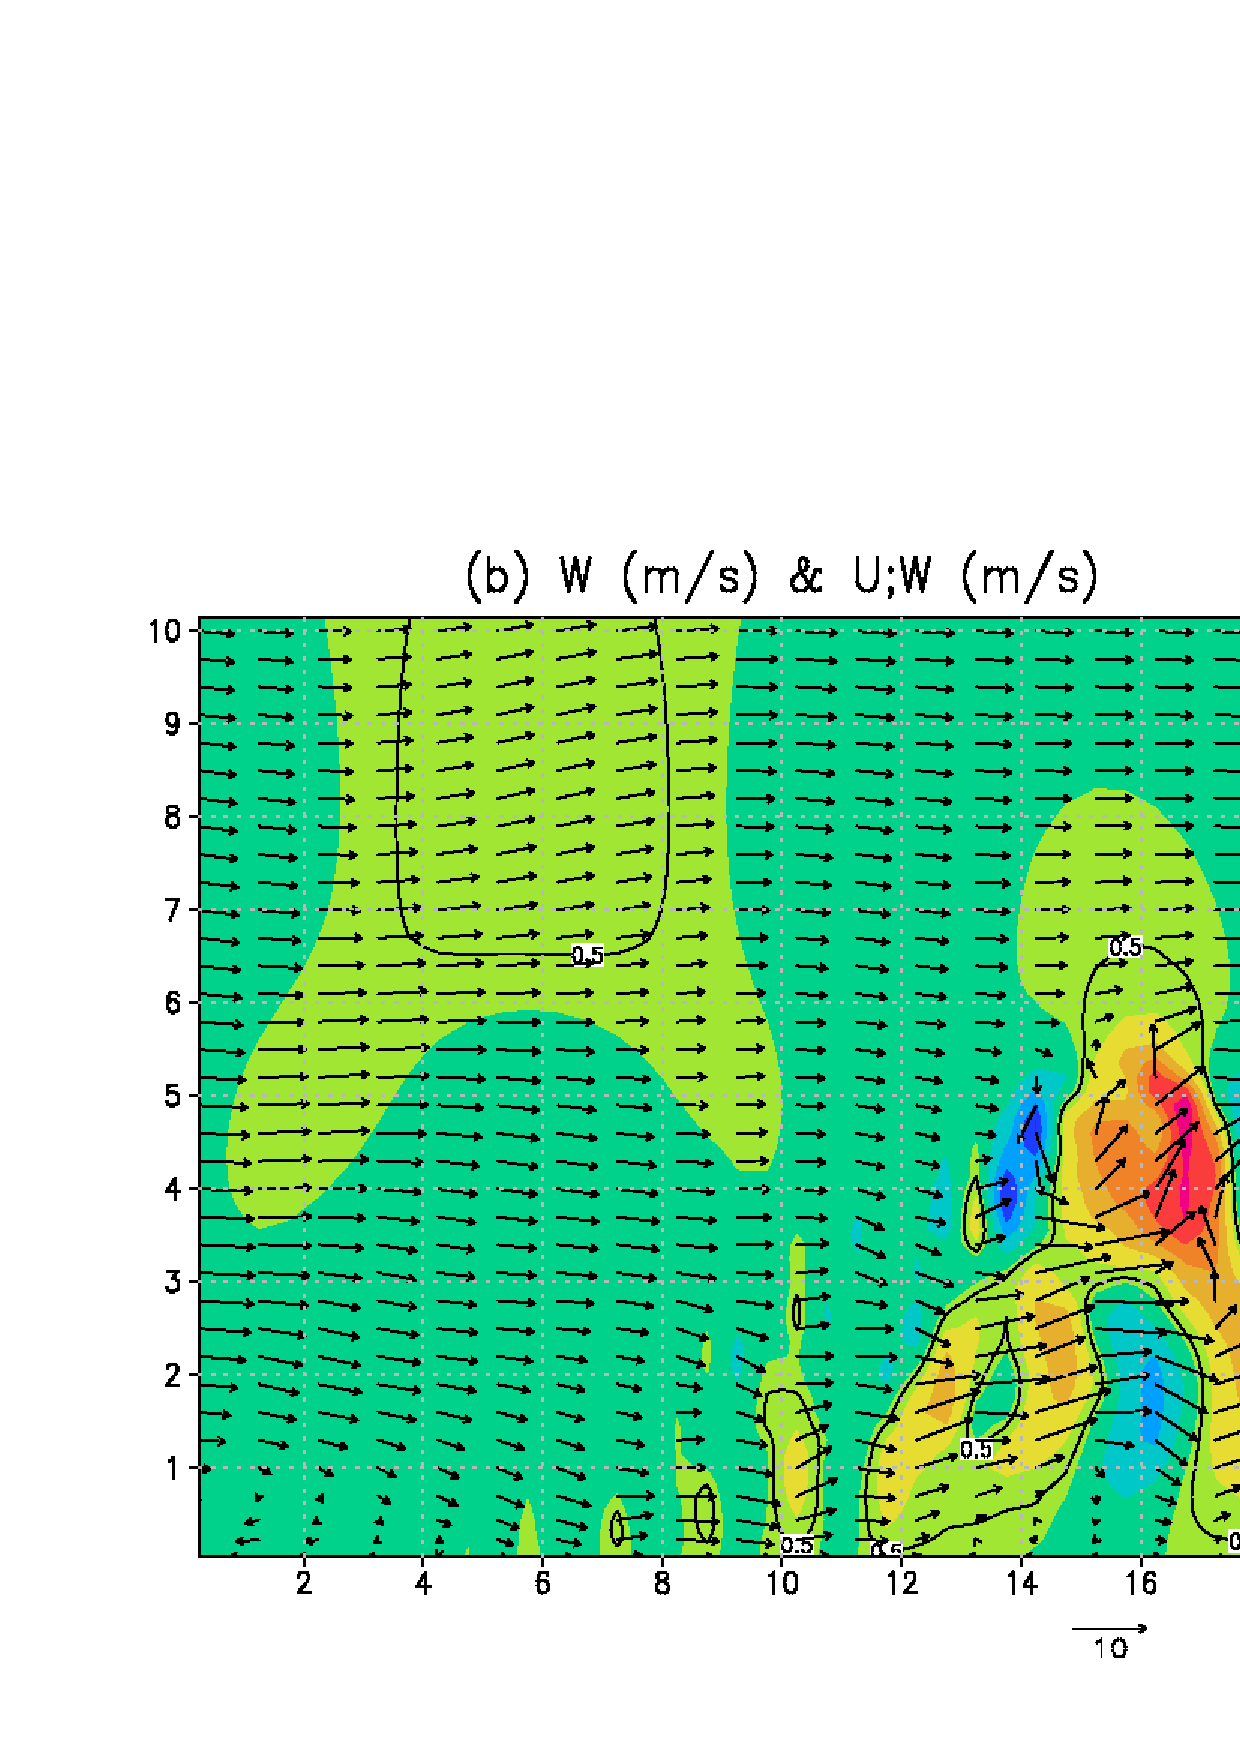
\includegraphics[width=0.7\hsize]{./figure/ideal_W.pdf}\\
  \caption{積分開始から 1200 秒(20 分)後の Y=750 mにおける東西-鉛直断面図;
           カラーシェードは、(a)において全質量に対する凝結物の質量比、
           (b)において鉛直速度を表す。ベクトルは東西-鉛直断面内の風の流れを表す。}
  \label{fig_ideal}
\end{center}
\end{figure}

他の変数もバイナリデータに変換したい場合は、
\verb|net2g_R20kmDX500m.conf|の\namelist{VARI}の\nmitem{VNAME} に必要な変数を追加すれば良い。
\editbox{
\verb|&VARI|\\
\verb| VNAME       = "U","W","QHYD"|\\
\verb|/|\\
}
ヒストリファイルに出力された変数は、{\netcdf} の\verb|ncdump| 等を
用いて簡単に確認できる。\verb|net2g|の詳しい使い方は第\ref{sec:net2g}節を参照されたい。
